% UCL Thesis LaTeX Template
%  (c) Ian Kirker, 2014
% 
% This is a template/skeleton for PhD/MPhil/MRes theses.
%
% It uses a rather split-up file structure because this tends to
%  work well for large, complex documents.
% We suggest using one file per chapter, but you may wish to use more
%  or fewer separate files than that.
% We've also separated out various bits of configuration into their
%  own files, to keep everything neat.
% Note that the \input command just streams in whatever file you give
%  it, while the \include command adds a page break, and does some
%  extra organisation to make compilation faster. Note that you can't
%  use \include inside an \include-d file.
% We suggest using \input for settings and configuration files that
%  you always want to use, and \include for each section of content.
% If you do that, it also means you can use the \includeonly statement
%  to only compile up the section you're currently interested in.
% You might also want to put figures into their own files to be \input.

% For more information on \input and \include, see:
%  http://tex.stackexchange.com/questions/246/when-should-i-use-input-vs-include


% Formatting rules for theses are here: 
%  http://www.ucl.ac.uk/current-students/research_degrees/thesis_formatting
% Binding and submitting guidelines are here:
%  http://www.ucl.ac.uk/current-students/research_degrees/thesis_binding_submission

% This package goes first and foremost, because it checks all 
%  your syntax for mistakes and some old-fashioned LaTeX commands.
% Note that normally you should load your documentclass before 
%  packages, because some packages change behaviour based on
%  your document settings.
% Also, for those confused by the RequirePackage here vs usepackage
%  elsewhere, usepackage cannot be used before the documentclass
%  command, while RequirePackage can. That's the only functional
%  difference.
\RequirePackage[l2tabu, orthodox]{nag}
\RequirePackage{amssymb}

% Required for writing algorithms
\RequirePackage[ruled]{algorithm2e}
%\renewcommand{\baselinestretch}{1.5}
\SetKwInput{KwInput}{Input}
%\newlength\algowd
%\def\savewd#1{\setbox0=\hbox{#1\hspace{.7in}}\algowd=\wd0\relax#1}
%\newcommand\algolines[2]{\savewd{#1}%
%  \tcp*{\parbox[t]{\dimexpr\algowidth-\algowd}{#2}}}

% ------ Main document class specification ------
% The draft option here prevents images being inserted,
%  and adds chunky black bars to boxes that are exceeding 
%  the page width (to show that they are).
% The oneside option can optionally be replaced by twoside if
%  you intend to print double-sided. Note that this is
%  *specifically permitted* by the UCL thesis formatting
%  guidelines.
%
% Valid options in terms of type are:
%  phd
%  mres
%  mphil
%\documentclass[12pt,phd,draft,a4paper,oneside]{ucl_thesis}
\documentclass[12pt,mres,a4paper,twoside]{ucl_thesis}


% Package configuration:
%  LaTeX uses "packages" to add extra commands and features.
%  There are quite a few useful ones, so we've put them in a 
%   separate file.
% -------- Packages --------

% This package just gives you a quick way to dump in some sample text.
% You can remove it -- it's just here for the examples.
\usepackage{blindtext}

% This package means empty pages (pages with no text) won't get stuff
%  like chapter names at the top of the page. It's mostly cosmetic.
\usepackage{emptypage}

% The graphicx package adds the \includegraphics command,
%  which is your basic command for adding a picture.
\usepackage{graphicx}

% This command is provided by the graphicx package, and 
%  controls the default dpi resolution of images you use.
%  72 is the default, but 300 is more normal, and 600 is
%  as good as you can expect to be able to get on normal paper.
\pdfimageresolution=300


% The float package improves LaTeX's handling of floats,
%  and also adds the option to *force* LaTeX to put the float
%  HERE, with the [H] option to the float environment.
\usepackage{float}

% The amsmath package enhances the various ways of including
%  maths, including adding the align environment for aligned
%  equations.
\usepackage{amsmath}

% Use these two packages together -- they define symbols
%  for e.g. units that you can use in both text and math mode.
\usepackage{gensymb}
\usepackage{textcomp}
% You may also want the units package for making little
%  fractions for unit specifications.
%\usepackage{units}


% The setspace package lets you use 1.5-sized or double line spacing.
\usepackage{setspace}
\setstretch{1.5}

% That just does body text -- if you want to expand *everything*,
%  including footnotes and tables, use this instead:
%\renewcommand{\baselinestretch}{1.5}


% PGFPlots is either a really clunky or really good way to add graphs
%  into your document, depending on your point of view.
% There's waaaaay too much information on using this to cover here,
%  so, you might want to start here:
%   http://pgfplots.sourceforge.net/
%  or here:
%   http://pgfplots.sourceforge.net/pgfplots.pdf
%\usepackage{pgfplots}
%\pgfplotsset{compat=1.3} % <- this fixed axis labels in the version I was using

% PGFPlotsTable can help you make tables a little more easily than
%  usual in LaTeX.
% If you're going to have to paste data in a lot, I'd suggest using it.
%  You might want to start with the manual, here:
%  http://pgfplots.sourceforge.net/pgfplotstable.pdf
%\usepackage{pgfplotstable}

% These settings are also recommended for using with pgfplotstable.
%\pgfplotstableset{
%	% these columns/<colname>/.style={<options>} things define a style
%	% which applies to <colname> only.
%	empty cells with={--}, % replace empty cells with '--'
%	every head row/.style={before row=\toprule,after row=\midrule},
%	every last row/.style={after row=\bottomrule}
%}


% The mhchem package provides chemistry formula typesetting commands
%  e.g. \ce{H2O}
%\usepackage[version=3]{mhchem}

% And the chemfig package gives a weird command for adding Lewis 
%  diagrams, for e.g. organic molecules
%\usepackage{chemfig}

% The linenumbers command from the lineno package adds line numbers
%  alongside your text that can be useful for discussing edits 
%  in drafts.
% Remove or comment out the command for proper versions.
%\usepackage[modulo]{lineno}
% \linenumbers 


% Alternatively, you can use the ifdraft package to let you add
%  commands that will only be used in draft versions
%\usepackage{ifdraft}

% For example, the following adds a watermark if the draft mode is on.
%\ifdraft{
%  \usepackage{draftwatermark}
%  \SetWatermarkText{\shortstack{\textsc{Draft Mode}\\ \strut \\ \strut \\ \strut}}
%  \SetWatermarkScale{0.5}
%  \SetWatermarkAngle{90}
%}


% The multirow package adds the option to make cells span 
%  rows in tables.
\usepackage{multirow}


% Subfig allows you to create figures within figures, to, for example,
%  make a single figure with 4 individually labeled and referenceable
%  sub-figures.
% It's quite fiddly to use, so check the documentation.
%\usepackage{subfig}

% The natbib package allows book-type citations commonly used in
%  longer works, and less commonly in science articles (IME).
% e.g. (Saucer et al., 1993) rather than [1]
% More details are here: http://merkel.zoneo.net/Latex/natbib.php
%\usepackage{natbib}

% The bibentry package (along with the \nobibliography* command)
%  allows putting full reference lines inline.
%  See: 
%   http://tex.stackexchange.com/questions/2905/how-can-i-list-references-from-bibtex-file-in-line-with-commentary
\usepackage{bibentry} 

% The isorot package allows you to put things sideways 
%  (or indeed, at any angle) on a page.
% This can be useful for wide graphs or other figures.
%\usepackage{isorot}

% The caption package adds more options for caption formatting.
% This set-up makes hanging labels, makes the caption text smaller
%  than the body text, and makes the label bold.
% Highly recommended.
\usepackage[format=hang,font=small,labelfont=bf]{caption}

% If you're getting into defining your own commands, you might want
%  to check out the etoolbox package -- it defines a few commands
%  that can make it easier to make commands robust.
\usepackage{etoolbox}


% Sets up links within your document, for e.g. contents page entries
%  and references, and also PDF metadata.
% You should edit this!
%%
%% This file uses the hyperref package to make your thesis have metadata embedded in the PDF, 
%%  and also adds links to be able to click on references and contents page entries to go to 
%%  the pages.
%%

% Some hacks are necessary to make bibentry and hyperref play nicely.
% See: http://tex.stackexchange.com/questions/65348/clash-between-bibentry-and-hyperref-with-bibstyle-elsart-harv
\usepackage{bibentry}
\makeatletter\let\saved@bibitem\@bibitem\makeatother
\usepackage[pdftex,hidelinks]{hyperref}
\makeatletter\let\@bibitem\saved@bibitem\makeatother
\makeatletter
\AtBeginDocument{
    \hypersetup{
        pdfsubject={Thesis Subject},
        pdfkeywords={Thesis Keywords},
        pdfauthor={Author},
        pdftitle={Title},
    }
}
\makeatother
    


% And then some settings in separate files.
% These settings are from:
%  http://mintaka.sdsu.edu/GF/bibliog/latex/floats.html

% They give LaTeX more options on where to put your figures, and may
%  mean that fewer of your figures end up at the tops of pages far
%  away from the thing they're related to.

% Alters some LaTeX defaults for better treatment of figures:
% See p.105 of "TeX Unbound" for suggested values.
% See pp. 199-200 of Lamport's "LaTeX" book for details.

%   General parameters, for ALL pages:
\renewcommand{\topfraction}{0.9}	% max fraction of floats at top
\renewcommand{\bottomfraction}{0.8}	% max fraction of floats at bottom

%   Parameters for TEXT pages (not float pages):
\setcounter{topnumber}{2}
\setcounter{bottomnumber}{2}
\setcounter{totalnumber}{4}     % 2 may work better
\setcounter{dbltopnumber}{2}    % for 2-column pages
\renewcommand{\dbltopfraction}{0.9}	% fit big float above 2-col. text
\renewcommand{\textfraction}{0.07}	% allow minimal text w. figs

%   Parameters for FLOAT pages (not text pages):
\renewcommand{\floatpagefraction}{0.7}	% require fuller float pages
% N.B.: floatpagefraction MUST be less than topfraction !!
\renewcommand{\dblfloatpagefraction}{0.7}	% require fuller float pages

% remember to use [htp] or [htpb] for placement,
% e.g. 
%  \begin{figure}[htp]
%   ...
%  \end{figure} % For things like figures and tables
\bibliographystyle{unsrt}   % For bibliographies

% Title Settings
\setcounter{secnumdepth}{3}
\setcounter{tocdepth}{3}
%\title{A Deep Reinforcement Learning Approach for Recommender Systems}
\title{Learning to Recommend using a Deep Reinforcement Agent}
\author{Hernan Santiago Gonzalez Toral}
\department{Department of Computer Science}
%\emailaddr{hernangt12re3@gmail.com}
\emailaddr{}
\supervisor{Dr. Jun Wang}
\supemail{jun.wang.l@cs.ucl.ac.uk}


\begin{document}



\nobibliography*
% This is a dumb trick that works with the bibentry package to let
%  you put bibliography entries whereever you like.
% I used this to put references to papers a chapter's work was 
%  published in at the end of that chapter.
% For more information, see: http://stefaanlippens.net/bibentry

% If you haven't finished making your full BibTex file yet, you
%  might find this useful -- it'll just replace all your
%  citations with little superscript notes.
% Uncomment to use.
%\renewcommand{\cite}[1]{\emph{\textsuperscript{[#1]}}}

% At last, content! Remember filenames are case-sensitive and 
%  *must not* include spaces.
\maketitle
%\makedeclaration

\begin{abstract} % 300 word limit
My research is about stuff.

It begins with a study of some stuff, and then some other stuff and things.

There is a 300-word limit on your abstract.
\end{abstract}

\begin{acknowledgements}
Acknowledge all the things!
\end{acknowledgements}


\setcounter{tocdepth}{2} 
% Setting this higher means you get contents entries for
%  more minor section headers.

\tableofcontents
\listoffigures
\listoftables


\chapter{Introductory Material}
\label{chapterlabel1}

Some stuff about things.\cite{example-citation} Some more things. 

Inline citation: \bibentry{example-citation}

% This just dumps some pseudolatin in so you can see some text in place.
\blindtext

\chapter{Background}
\label{chapterlabel2}

\section{Recommender Systems}

use background patterns of \textbf{An MDP-Based Recommender System} 

\subsection{Matrix Factorization}

In a recommendation system such as Netflix or MovieLens, there is a group of users and a set of items (movies for the above two systems). Given that each users have rated some items in the system, we would like to predict how the users would rate the items that they have not yet rated, such that we can make recommendations to the users

the task of predicting the missing ratings can be considered as filling in the blanks such that the values would be consistent with the existing ratings in the matrix.

The intuition behind using matrix factorization to solve this problem is that there should be some latent features that determine how a user rates an item. Hence, if we can discover these latent features, we should be able to predict a rating with respect to a certain user and a certain item, because the features associated with the user should match with the features associated with the item.

In trying to discover the different features, we also make the assumption that the number of features would be smaller than the number of users and the number of items

we have a set U of users, and a set D of items. Let $\mathbf{R}$ of size $|U| \times |D|$ be the matrix that contains all the ratings that the users have assigned to the items. Also, we assume that we would like to discover K latent features. Our task, then, is to find two matrics matrices $\mathbf{P}$ (a $|U| \times K$ matrix) and $\mathbf{Q}$ (a $|D| \times K$ matrix) such that their product approximates $\mathbf{R}$:

\begin{equation}
\label{}
\mathbf{R} \approx \mathbf{P} \times \mathbf{Q^{T}} = \hat{\mathbf{R}}
\end{equation}

Each row of $\mathbf{P}$ would represent the strength of the associations between a user and the features. Similarly, each row of $\mathbf{Q}$ would represent the strength of the associations between an item and the features. We have to find a way to obtain $\mathbf{P}$ and $\mathbf{Q}$. One way to approach this problem is the first intialise the two matrices with some values, and calculate how 'different? their product is to $\mathbf{M}$ by using gradient descent with a regularization term in order to find the minimum difference between $\mathbf{R}$ and the predicted preference matrix $\mathbf{\hat{R}}$ (using the MSE).The update rules and the cost function are defined as follows:

\begin{equation}
\label{}
p^{'}_{ik}=p_{ik}+\alpha\frac{\partial}{\partial p_{ik}}e^{2}_{ij}=p_{ik}+\alpha(2e_{ij}q_{kj}-\beta p_{ik})
\end{equation}

\begin{equation}
\label{}
q^{'}_{kj}=q_{kj}+\alpha\frac{\partial}{\partial q_{kj}}e^{2}_{ij}=q_{kj}+\alpha(2e_{ij}p_{ik}-\beta p_{kj})
\end{equation}

\begin{equation}
\label{}
e^2_{ij}=(r_{ij}-\hat{r{ij}})^2=(r_{ij}-\sum_{k=1}^{K}p^{'}_{ik}q^{'}_{kj})^2
\end{equation}

\section{Reinforcement Learning}

as a reinforcement learning task called the multi-armed bandit [Sutton and Barto 1998]

Reinforcement learning involves modifying the behavior of a system such that the expected value of some possibly delayed scalar feedback is maximized.

Reinforcement learning [7, 19] is a family of machine learning algorithms that optimize sequential decision making
processes based on scalar evaluations called reinforcements. The objective is to maximize the expected sum of future reinforcements for each state.

If for each state the best action is taken according to the estimated value function, then the policy is called greedy.

An MDP is a model for sequential stochastic decision problems where an autonomous agent is influencing its surrounding environment through actions

For categorizing RL agents, base the writing on the definition of approaches to approximate the optimal policy in \textbf{DJ-MC: A Reinforcement-Learning Agent for Music Playlist Recommendation}

Q-Learning in which values are estimated for each state and action combination

Exploration/Exploitation
exploitation corresponds with the generation of trust and the exploration with the presentation of new and unexpected items

the exploitation makes the behavior of the users more predictable, making estimates of the values more reliable. The exploration makes sure that the users have a chance to visit all pages, since it allows for all alternatives to be tried



\section{Recommender Systems and Reinforcement Learning}

**References to papers are temporarily described with their title in order to facilitate the identification of the source, but they will be replaced with proper latex references 

The first experiments on using reinforcement learning techniques were focused on developing recommendation systems for web content and using implicit data from server log files which stored the navigation of the users throughout their contents.

\textbf{Exploration/Exploitation in Adaptive Recommender Systems} considered reinforcement learning with an exploration/exploitation approach of unknown areas to automatically improve their recommendation policy for helping users to navigate through an adaptive web site. They state that a model-free algorithm like Q-Learning can become infeasible if the number of actions are so high. Additionally, they showed that a greedy policy can indeed lead to a suboptimal recommendation model as the use of such kind of policy function, where the \"best\" actions (e.g with higher probability) are taken, does not always improve the policy, so to avoid reinforcing values for states with initial high values, a random exploration process needs to be added to the action selection. The popular exploration $\epsilon$ greedy policy algorithm which modifies the action selection by selecting a greedy action with probability ($1-\epsilon$) or an arbitrary action with probability $\epsilon$ otherwise in order to explore  other existing options for the user. However, the exploration/exploitation dilemma came out as the exploration makes the future of a sequence less predictable influencing the estimation of the value function itself but inconsistent random actions have to be chosen to obtain a better policy. They finally demonstrated that this problem is solved by starting the algorithm with a lot of exploration and gradually reduce the parameter $\epsilon$ when the policy is getting closer to the optimum. Results concluded that a recommender system without exploration potentially can get trapped into a local maxima.

\textbf{New Recommendation System Using Reinforcement Learning} presented a general framework for web recommendation that learns directly from customer's past behavior by applying an RL process which uses the SARSA method[***ref here] and a $\epsilon$-greedy policy. The system was composed of two models: a global model to keep track of customers trends as a whole, and a local model to record the user's individual browsing history. In general, the model treats pages as states of the system and links within a page as actions. To predict the next state, it used a ranking system that is also separated into 2 parts. i) a global ranking system using the data from a $Q_{global}$-matrix obtained from the action-value function to choose the next state by applying an $\epsilon$-greedy policy. It gave the chance for rank new items that have few clicks but may match a user's interest. ii) a local ranking $Q_{local}$ which uses an inverse $\epsilon$-greedy policy to estimate the next state. It gave to customers more chance to explore other products than the ones they already visited. As a result, the system finds the final total reward using  $Q_{total}=Q_{local} + wQ_{global}$ where $w \in (0-1]$ is a weight hyper parameter of the model.

Authors performed some experiments to find a relationship between $\epsilon$ and the user click rate. The findings showed that a value of $\epsilon=0.2$ preserves the balance between exploration and exploitation, meanwhile If $\epsilon < 0.2$ the system will gave small chances to users to explore new items, or may include products that do not match to the customer's interest otherwise ($\epsilon > 0.2$). Even if the purpose of $Q_{local}$ was to promote new products, it was less effective than $Q_{global}$. In conclusion, the result of this experiments explained that if a user is allowed to do much exploration, she has a chance to find non-relevant products, but if users just exploit the system, they have a chance to just keep receiving the same recommended items over time.

\textbf{An MDP-Based Recommender System} argue that it is more appropriate to formulate the problem of generating recommendations as a sequential optimization problem so they described a novel approach for a commercial web site based on Markov Decision Processes (MDPs) together with a novel predictive model that outperformed previous models. An MDP-based recommender system can take into account the expected utility and the long-time effect of a particular recommendation, and suggest an item whose immediate reward is lower, but leads to more \textit{profitable} rewards in the future. Moreover, these considerations are taken into account automatically by any optimal policy generated for an MDP model which ensures a balance in the generation of the maximal expected reward stream. However, the previous benefits are offset by the fact that the model parameters are unknown, randomly initialized and that they take considerable time to converge. So, they introduced in their work a model-based system for collaborative filtering with a strong initial model, which solves quickly, and that does not consume too much memory.

Before implementing the recommender, they initialize a predictive model of user behavior using data extracted from the web site, and then use it to provide the initial parameters for the MDP. The predictive model can be thought of as a first-order Markov chain (MC)[***] of user dynamics in which states correspond to sequences of \textit{k} events (in this case: previous selections) representing relevant information about the users interaction. They experimented with small values of \textit{k} ($k \in [1-5]$) in order to overcome data sparsity and MDP solution complexity issues. Thus, the transition function describes the probability that a user whose \textit{k} recent selections were $x_1, . . . ,x_k$ will select the item $x'$ next. Finally, enhancements on the maximum-likelihood n-gram formulation[***] were proposed in order to find a good estimate of the transition function for the initial predictive model without suffering the problem of data sparsity and bad performance.

The proposed maximum-likelihood estimation include three major enhancements. First, a form of skipping based on the observation that the occurrence of the sequence $x_1,x_2,_x3$ lends some likelihood to the sequence $x_1,x_3$. In other words, after initializing the counts of each state transition using the observed data, for any given user sequence $x_1,x_2, ...,x_n$, they added a fractional count $1/2^{( j-(i+3))}$ to the transition from $s=\langle x_i,x_{i+1},x_{i+2}\rangle$ to $s'=\langle x_{i+1},x_{i+2},x_j\rangle$, for all $i+3 < j ?n$, which acts as a diminishing probability of skipping a large number of transactions in the sequence. Equation \ref{eq:trMCSkipping} shows the updated formulation of the (normalized )maximum-likelihood estimation, where $count(s,s')$ is the fractional count associated with the transition from s to s'.

\begin{equation}
\label{eq:trMCSkipping}
tr_{MC}^{base}(s,s')=\frac{count(s, s')}{\sum_{s'}count(s, s')}
\end{equation}

The second enhancement exploits the similarity  of sequences in a form of clustering. The idea is that the likelihood of transition from $s$ to $s'$ can be predicted by occurrences from $t$ to $s'$, where $s$ and $t$ are similar. Equation \ref{eq:simTr} define the similarity of states $s_i$ and $s_j$ where $\delta(\dot, \dot)$ is the Kronecker delta function and $s^m_i$ is the m-th item in state $s_i$. Then, the similarity count from state $s$ to $s'$ was defined using equation \ref{eq:simCountTr}. Finally, the new transition probability from $s$ to $s'$ given by equation \ref{eq:newTr} yielded the best results during evaluation.

\begin{equation}
\label{eq:simTr}
sim(s_i, s_j)=\sum_{m=1}^{k}\delta(s_i^m, s_j^m) \cdot (m+1)
\end{equation}
\begin{equation}
\label{eq:simCountTr}
simcount(s, s')=\sum_{s_i} sim(s, s_i) \cdot tr^{base}_{MC}(s, s')
\end{equation}
\begin{equation}
\label{eq:newTr}
tr_{MC}(s, s')=\frac{1}{2}tr^{base}_{MC}(s, s') + \frac{1}{2}\frac{simcount(s, s')}{\sum_{s''}simcount(s, s'')}
\end{equation}

Due to larger values of k lead to states that are more informative whereas smaller values of k lead to states with more statistical meaning, they added as a third enhancement a finite mixture modeling (e.g. combine a trigram, a bigram and a unigram into a single model) in a way to balance these conflicting properties by mixing k models, where the \textit{i-th} model looks at the last i transactions. In addition, they applied mixture weights during experiments as $\pi_1 = � � � = \pi_k = 1/k$ so the generation of the models for smaller values entails little computational overhead.

An evaluation on the accuracy of the predictive model was performed using real user transactions and browsing paths (from web logs) from the commercial store web site. Besides, they compared different variations of their enhancements on the MC approach with other models like i)both sequential and non-sequential form of the \textit{Microsoft Commerce Server 2000}(Heckerman et al. (2000))[***] (local distributions are probabilistic decision trees); and ii)unordered versions of MC models. Results outlined that the MC models using skipping, clustering, and mixture modeling yielded better results than any other other variation of model \textit{i}. Sequence-sensitive models outperformed the accuracy of non-sequential models, while MC models were superior to the predictor models. and the skipping enhancement was only beneficial for the transactions data set

On the other hand, the MDP-based recommender system, models the recommendation process as a sequence of states and attempts to optimize it. Here, the predictive model played an important role in the construction of the model as it provides the probability, denoted by $Pr_{pred}(x|x_1, . . . ,x_k)$, that a user purchase a particular item x given her sequence of past purchases  $x_1, . . . ,x_k$. The components of the reinforcement learning model are defined as follows: a) the states are the \textit{k}-tuples of items purchased; b) the actions correspond to a recommendation of an item; c) the rewards depends on the last item defining the current state only, where its net profit of the item was used; and d) the transition function is the stochastic element of the model and estimates the user's actual choice. In brief, equation \ref{eq:trMDP} represents the transition function or the probability that a user will select item $x''$ given that item $x'$ is recommended in state $\langle x_1,x_2,x_3 \rangle$.

\begin{equation}
\label{eq:trMDP}
tr^1_{MDP}(\langle x_1,x_2,x_3 \rangle,x',\langle x_2,x_3,x'' \rangle) 
\end{equation}

In order to solve the MDP, the policy iteration algorithm was used as their state space enjoys of the following features that lead to fast convergence: i) the inherent directionality that transitions showed are useful to reduce the running time of the solution algorithm; ii) the computation of an optimal policy is not sensitive to variations in the number of \textit{k} past transactions a state represent; iii) ignoring unobserved states by maintaining transition probabilities only for states where a transition actually occurred; and  iv) using the independence of recommendations or Markov property, where the probability that a user buys a particular item depends only on her current state, allowing the algorithm to handle large action spaces.Tests performed on real data showed that the policy iteration converges after a few iterations.

To update the model, the system used an off-line approach which keeps track of the recommendations and the user selections and build a new model at fixed time intervals (e.g. once a week). So, to re-estimate the transition function at time $t+1$ the following counts are obtained:

\begin{equation}
\label{eq:countIn}
c^{t+1}_{in}(s, r, s \cdot r) = c^{t}_{in}(s, r, s \cdot r) + count(s, r, s \cdot r)
\end{equation}
\begin{equation}
\label{eq:countOut}
c^{t+1}_{out}(s, r, s \cdot r) = c^{t}_{out}(s, r, s \cdot r) + count(s, s \cdot r) - count(s, r, s \cdot r)
\end{equation}
\begin{equation}
\label{eq:countTotal}
c^{t+1}_{total}(s, s \cdot r) = c^{t}_{total}(s, r, s \cdot r) + count(s, s \cdot r)
\end{equation}
\begin{equation}
\label{eq:modelProb1}
tr(s, r \in R, s \cdot r) = \frac{c^{t+1}_{in}(s, r, s \cdot r)}{c^{t+1}_{total}(s, s \cdot r)}
\end{equation}
\begin{equation}
\label{eq:modelProb2}
tr(s, r \notin R, s \cdot r) = \frac{c^{t+1}_{out}(s, r, s \cdot r)}{c^{t+1}_{total}(s, s \cdot r)}
\end{equation}
\begin{equation}
\label{eq:initIn}
c^{0}_{in}(s, r, s \cdot r) = \xi_S \cdot tr(s, r, s \cdot r)
\end{equation}
\begin{equation}
\label{eq:initOut}
c^{0}_{out}(s, r, s \cdot r) = \xi_S \cdot tr(s, r, s \cdot r)
\end{equation}
\begin{equation}
\label{eq:initTotal}
c^{0}_{total}(s, s \cdot r) = \xi_S 
\end{equation}
where Equation \ref{eq:countIn} corresponds to the number of times a recommendation r was accepted in state s, equation \ref{eq:countOut} is the number of times a user select item r in state s even though it was not recommended, equation \ref{eq:countTotal} is the number of times a user pick item r while being in state s, regardless of whether it was recommended or not, and finally, equations \ref{eq:modelProb1} and \ref{eq:modelProb2} represent the actual probability that a user will select item r given state s when r was recommended or not respectively. 

The transition function had to be carefully initialized in order to be fairly accurate when the system was first deployed to avoid the cold-start problem, so the at time $t=0$ were calculated using equations \ref{eq:initIn} \ref{eq:initOut} \ref{eq:initTotal}, where $\xi_s= 10 \cdot count(s)$, causing states that are infrequently observed to be updated faster than already observed states. Moreover, when the first transition to a state $s \cdot r$ is observed, its probability is initialized to 0.9 the probability of the most likely next item in state s with $\xi_s =10$. In this way, the system balances the need to explore unobserved items in order to improve its model by recommending non-optimal items occasionally until getting their actual counts. 

Finally, an empirical validation of their thesis compared the performance in terms of their value or utility and computational cost of the MDP-based recommender system with the performance of a recommender  based on the predictive model (MC) as well as other variants. The deployed system was built using three mixture components (combined using an equal weight), with history length $k \in [1,3]$ for both the MDP and MC model, and used the policy-iteration procedure and approximations. The average profit generated by users using the site was 28\% higher for the MDP group. while in terms of computational costs, the MDP-based model provided fastest recommendations at the price of more memory use, and also built models more quickly. 

All in all, the approach presented make use of off-line data to initialize a model in order to provide an adequate initial performance and overcome the cold-start problem, the authors avoid using some form of reinforcement learning technique as they argue that its implementation requires many calls and computations by a recommender system online, which will lead to slower responses, producing undesirable results for the web site owner.

\textbf{Usage-Based Web Recommendations: A Reinforcement Learning Approach} proposed a machine learning perspective based on a off-line reinforcement learning model to solve the recommendation problem using the Q-Learning algorithm while employing concepts and techniques commonly applied in the web usage mining domain. They argued that their decision on using this method seems appropriate for the nature of web page recommendation problem
as it provides a mechanism which is constantly learning, does not need periodic updates, can be easily adapted to changes in the website structure and new trends in users behavior. Consequently, the system was trained using web usage logs available as the training set and experimental evaluations were carried out in order to demonstrate how this approach can improve the quality of web recommendations.

The RL problem formulation was considered as as a competition between different recommender systems to gather more points, than a 2-player game, as in the recommender system environment, self-play, a typical technique used in training RL systems[***], cannot be used to train the system so the system needed of actual web usage data for training. Moreover, the model, which has a stochastic nature, consists of the following properties: 

\textbf{states:} showing the history of pages visited by the user so far. For this case, a notion of N-Grams was adopted and a sliding window of size $w$ was set to limit the page visit sequences to a constant number and avoid large state spaces.

\textbf{actions:} consists of a single page recommendation at each state.

\textbf{policy:} computes the reward of performing an action a in state s. It rewards actions positively if it recommends a page that will be visited in one of the consequent states (not necessarily the immediate next state). Formally, rewards are dependent on the next state, the intersection of previously recommended pages in each state and the current page sequence of the state. 

As the model does not have a predetermined reward function $R(s, a)$ or a transition function $\delta(s, a)$ to give the next state, the reward can be estimated by considering each state s is formed by two sequences $V_s =\langle p^V_{s,1}, p^V_{s,2},..., p^V_{s,w} \rangle$, and $R_s =\langle p^R_{s,1}, p^R_{s,2},..., p^R_{s, n} \rangle$, indicating the sequence of visited and previously recommended pages respectively, where $p^V_{s, i}$ , indicates the ith visited page in the state and $p^R_{s, i}$ indicates the ith recommended page in the state s, Additionally, they had two considerations in the implementation of the reward function: i) only the occurrence of the last page visited in the recommended pages list in state $s'$ is used to reward the action performed in the previous sate $s$, and ii) the time the user spends on a page, assuming that the more time a user spends on a page the more interested. So, the reward function was defined as follows:
\begin{enumerate}
\item Assume $\delta(s, a) = s'$
\item $P_R = V_{s', w} \cap R_{s'}$
\item if $p \neq \emptyset$
\item For page $p$ in $P_R$
\begin{enumerate}
\item $r(s, a) += reward(Dist(Rs', p), Time(p^v_w))$
\end{enumerate}
\end{enumerate}
where $Dist(R_i, p)$ is the distance of page p from the end of the recommended pages list and $Time(p^v_w)$ indicates the time user has spent on the last page of the state. Finally, The $reward(Dist, Time)$ function was defined as a linear combination of both values as $reward(Dist,  Time) = \alpha \times dist + \beta \times Time$ with $\alpha + \beta = 1$.

Subsequently, the  definition of the learning algorithm also took into consideration the following characteristics: 1) the Q-Learning algorithm given by equation \ref{eq:QLearningalg} was proposed as an update rule and the structure to estimate how successful a prediction can be. Here, the decreasing value of $\alpha_n$ caused these values to gradually converge and decreases the impact of changing reward values as the training continues; 2) an $\epsilon$-greedy action selection was picked as it is important to add some exploration of the state space especially at the beginning of the training; 3) the algorithm followed a TD(0) off-policy learning[***] procedure, as the maximum Q value of the next state is considered when estimating the future reward; and 4) the computation of $r(s, a)$ suffered a slightly change by considering value of $Q(s',a)$ with a coefficient $\gamma$ in order to propagate the value of performing a specific action beyond the limits imposed by the $w$. As the authors mentioned in their work: "the basic idea is that when an action/recommendation is appropriate in state Si, indicating the recommended page is likely to occur in the following states, it should also be considered appropriate in state $S_{i-1}$ and the actions in that state that frequently lead to $S_i$". During the training phase, the described algorithm converged after a few thousand (between 3000 and 5000) visits of each episode or user session.

\begin{equation}
\label{eq:QLearningalg}
Q_n(s, a )= [(1 - \alpha_n)Q_{n-1}(s, a) + \alpha_n[r(s, a)  + \gamma \max_{a'} Q_{n-1}(\delta(s, a), a')]
\end{equation}
with
\begin{equation}
%\label{}
\alpha_n = \frac{1}{1 + visits_n(s, a)}
\end{equation}

For the purpose of performing a set of experimental evaluations of the proposed model, simulated log files generated by a web traffic simulator were used to train and tune the rewarding functions. The metric used for each evaluation were Recommendation Accuracy, Coverage (similar to precision and recall metrics) and Shortcut Gain (measures how many page-visits users can save if they follow the recommendations). First of all, an experiment with different values of $w$ showed that fixed window size of 3 as recommendation history resulted on better accuracy and shortcut gain, so this value was set for the rest of system evaluations. Next, they experimented the impact of gradually increasing (in steps of 5\%) the coefficient $\alpha$ of parameter \textit{Dist} in the reward function, resulting on both higher accuracy and higher shortcut gain for values up to 15\%. This matched the natural consequence of adding a bounded size of window on recommendations history. Finally, a set of experiments also tested the system performance by increasing the coefficient $\gamma$ in the reward function, obtaining an increase of the accuracy until reaching an upper bound (around 0.20\%) where it began to drop, while the shortcut gain increased steadily up to a point where recommendations became so inaccurate.

Briefly, the proposed off-line reinforcement learning method used a simple formulation of the recommendation problem but it obtained much better results compared with two baselines methods: association rules and item-based collaborative filtering (with probabilistic similarity measure). As the coverage increased, naturally accuracy decreased in all systems, but the RL approach outperformed the other two systems displaying a lower rate in which its accuracy decreased. Authors concluded that the algorithm is a good candidate for solving the recommendation problem as it does not rely on any previous assumptions regarding the probability distribution of visiting a page after having visited a sequence of pages, and that the nature of the problem matches perfectly with the notion of delayed reward (known as temporal difference). In addition, they suggested that it could be possible to use a more complicated formulation of the reward function rather than a linear combination of factors, such as a neural networks, in order to produce better results.

Later, in \textbf{A Hybrid Web Recommender System Based on Q-Learning} they exploited the previous reinforcement learning framework and present a hybrid web recommendation method enriched with semantic knowledge about the usage behavior as a way to improve the RL solution and obtain a more generalized solution regarding to the usage data it has. The new system used the incremental DCC[***] clustering algorithm to map pages to higher level concepts, and thus exploit the hierarchical and conceptual document clustering to provide a semantic relationship between them in combination with the usage data in a user session. Therefore, each state now consists of a sequence of concepts visited by the user, while actions are recommendation of pages that belong to a specific concept. This definition resulted in a much smaller state-action space as the size of the state space is now dependent on the number of distinct page clusters.

Now, an action $a$ recommending a concept $c$ is rewarded if the user visits a page belonging to concept $c$ later in his browsing session. The new reward function shown in  equation \ref{eq:hybridreward} takes into account the content similarity of the recommended and visited pages, where CBR represents the content-based reward of an action (which is equal to the similarity score between concepts) defined in equation \ref{}, and UBR is the usage-based reward defined in the previous approach.

\begin{equation}
\label{eq:hybridreward}
UBR(Dist(R_{s'} , r),Time(P_{t+1})) \times CBR(r, C(P_{t+1}))
\end{equation}
\begin{equation}
\label{}
l(c) = -log \mathcal{p}(c)
\end{equation}
\begin{equation}
\label{}
Sim(c_1, c_2) = max_{a \in LCA} {l(a)}
\end{equation}

To sum up, the algorithm did not make predictions based on weak usage patterns as now the states represent a generalized view of many single visit sequences. However, this approach seems specifically appropriate for the off-line training phase. On the other hand, evaluation results showed the flexibility of the new RL approach to incorporate different sources of information to improve the quality of recommendations, and also demonstrated how it could be extended in order to incorporate various sources of information.

\textbf{Improving adaptation of ubiquitous recommender systems by using reinforcement learning and collaborative filtering} proposed a learning system for Context-based Recommender System (CBRS)[***] by modeling an MDP agent which combines a hybrid Q-learning algorithm (HQL), collaborative filtering and case-based reasoning techniques in order to define a \textit{contextual} recommendation process based on different context dimensions (cognitive, social, temporal, geographic). It addressed the following problems that came out in recommender systems: a)avoid the intervention of experts as the use of the Q-learning algorithm does not need initial user?s information; b)reduce the cold start problem thanks to the ability of the Q-learning algorithm to explore the knowledge of other users in the same context by using CF; c)accelerate the learning process by mixing Q-learning with case-based reasoning techniques (reuse of cases yields to faster user satisfaction); and d)an exploration strategy allows recommendations to adapt to the user's interest evolution.

As a result, the model was based in three main algorithms. First, a hybrid-based CF approach which combines the advantages of the memory-based (fill the missing rating values of the user-item matrix) and model-based CF (form the nearest neighbors of each item). Second, the Case based reasoning (CBR)[***] algorithm was picked as it uses knowledge of previous cases to solve new problems, by finding a similar past case and thus reusing it to solve the current situation. Finally, the Q-learning algorithm was improved by: i)reusing past cases information gathered from the CBR, and ii)giving the ability to use information from other users sharing the same interests, by extending the $\epsilon$-greedy strategy to select a random action based on the similarity of user profiles (obtained from the CF algorithm).

The global mechanism of a context-based recommender system (CBRS) which uses the HyQL algorithm was composed mainly by the following modules:

\textbf{sensing module:} detects time, location, cognitive and social dimensions of the context.

\textbf{thinking module:} composed by an abstraction phase that is based on inference rules defined on temporal and space ontologies, and an aggregation phase the two dimensions.

\textbf{reasoning module:} chooses an action based on the HyQL algorithm

Finally, evaluations comparing the Q-learning and HyQL with respect to solving the cold start problem were performed, and consisted on testing the precision of the first 100 trials of the system starting when the user is connected to the system. In General, results showed that the precision of HyQL was greater than the precision of Q-learning, demonstrating that this approach is a good candidate to be used in the recommender system problem. However, as the system implementation depends on the context data, it needs of a hand-crafted feature creation process in order to be used on different situations.

\textbf{Exploration in Interactive Personalized Music Recommendation: A Reinforcement Learning Approach} formulated an interactive and personalized music recommendation approach as a reinforcement learning task based on the multi-armed bandit problem, where songs were treated as arms and user ratings as payoffs, and the objective function was set to maximize the cumulative reward of a targeted user over the long term. The model considered the exploration-exploitation trade-off and a Bayesian model in order to deal with both audio content and the novelty of recommendations and thus learn the user musical preferences online based on their feedback. 

The model differs from other approaches in three aspects: i)it is based on audio content; ii)the model is highly efficient as it allows easy online updates; and iii)the model is evaluated based on online real-life user interaction data and does not need a test dataset. Moreover, each recommendation serves two objectives: (1) satisfy the user?s current musical taste, and (2) obtain user feedback needed to improve future recommendations. Even though authors mentioned that an MDP formulation can model a broader range of problems than the multi-armed bandit, it requires much more data to train and is often more computationally expensive.

Their choice to work with a the content-based approach rather CF was justified for the following reasons. First, due to the bayesian nature of their formulation, methods for matrix factorization (MF) are much more complicated than the proposed linear model. Second, MF often needs of large amount of data for training. Third, existing Bayesian MF methods are inefficient for online updating, so they do not fit in a bandit model which is updated once a new rating is obtained, Fourth, a content-based method does not suffer of the new song problem. Finally, content-based approaches capture causality within music content rather than pure correlation that CF methods offer.

Subsequently, the interactive, personalized recommender system used a reinforcement learning task called the multi-armed bandit[***] which addressed both the exploration-exploitation trade-off and playlist generation with a single unified model. Whereas some RL models considered only a greedy strategy that does not actively seek fort user feedback, resulting in suboptimal recommendations over the long term, this model takes into account the uncertainty of both the mean and the variance of the rating distribution, allowing the recommender to explore user preferences actively rather than merely exploiting the available rating information. An approach better than the typical $\epsilon$-greedy method to solve of the multi-armed bandit problem, is the use of the Upper Confidence Bound (UCB)[***] algorithm, but it requires an explicit form of the confidence bound that is difficult to derive in the case of music recommendation.

The personalized music rating model was focused on audio content and novelty. The former considers the overall preference of a song and is represented by the linear function $U_c = \mathbf{\theta'x}$ where $\mathbf{x}$ is the feature vector of the audio content and $\mathbf{\theta}$ is the user preference in different music features (it was considered constant over time). On the other hand, the novelty factor was defined after examining the song's repetition distribution of 1000 users? listening histories collected from the Last.fm dataset. Results showed that most of the songs a user listens to are repeats and that the frequency distribution approximately follows the Zipf?s law[***], where only a small set of songs are repeated most of the time. As a consequence, it was assumed that the novelty of a song decays immediately after it is listened to and then gradually recovers according to the function $U_n = 1 - e^{-t/s}$, where s is a recovery speed (unknown) parameter learned from user interactions and $e^{-t/s}$ is the well-established forgetting curve[***] that measures user's memory retention of a song. In other words, novel songs are those of which that at a certain time a user has little or no memory. It is important to emphasize that the definition of this factor could be different or not applicable to other recommendation contexts than the musical environment.

Overall, the rating model, defined in equation \ref{eq:combinedRatingModel}, assumed that a rating is formed as the combination of the user?s preference of the song?s content and the dynamically changing novelty. Hence, each user was represented by a set of parameters $\Omega = \{\theta, s\}$, where $\Omega$ needs to be estimated from historical data, so uncertainty had to be taken into account. 

\begin{equation}
\label{eq:combinedRatingModel}
U = U_cU_n = \mathbf{\theta'x}(1 - e^{-t/s})
\end{equation}

With this in mind, the new problem formulation was solved using the Bayesian Upper Confidence Bound (Bayes-UCB)[***] algorithm. In The Bayes-UCB, the true expected payoff $U_i$ defined in equation \ref{eq:expectedRatingUCB} for arm \textit{i} is treated as a random variable and the posterior distribution $p(U_i|\mathcal{D})$ of $U_i$ given the history of payoffs $\mathcal{D_l} = \{(\mathbf{x_i}, t_i, r_i)\}^{l}_{i=1}$ is predicted using equations\ref{eq:posteriorDistrOmega} and \ref{eq:posteriorDistrU}. Finally, the Bayes-UCB recommends song $k^*$ that maximizes the quantile function $argmax_{k=1...|S|} Q(\alpha, P(U_k|D_l))$ where Q satisfies$\mathcal{P}[Uk \leq Q(\alpha, P(U_k|D_l))] = \alpha$ and $\alpha = 1 - \frac{1}{l+1}$

\begin{equation}
\label{eq:expectedRatingUCB}
\mathcal{E}[R_i] = U_i = \mathbf{\theta'x_i}(1 - e^{-t_i/s})
\end{equation}
\begin{equation}
\label{eq:posteriorDistrOmega}
p(\mathbf{\Omega}|D_l) \propto p(\mathbf{\Omega}) p(\mathbf{\Omega}|D_l)
\end{equation}
\begin{equation}
\label{eq:posteriorDistrU}
p(U_k|D_l) = \int p(U_k|\mathbf{\Omega}) p(\mathbf{\Omega}|D_l) \mathbf{d\Omega}
\end{equation}

Since equation \ref{eq:posteriorDistrOmega} does not have a closed-form solution, a Markov Chain Monte Carlo (MCMC)[***] should be used as an approximate inference algorithm. However, authors argued that its performance is very low and users could wait for up to a minute until the MC converges. Hence, they developed a Bayesian model using a piecewise-linear function approximation, as well as a variational inference algorithm to approximate posterior distribution of $\Omega$. For more details about the model definition, please refer to section 4.2 in [***](this paper). Authors mentioned that even if the model just considered audio content and novelty of music on its definition, other factors like diversity, mood or genre could be also approximated by linear functions and then added to it. All in all, the defined approximate Bayesian model was used to obtain the fixed-level quantile of $p(U_i|\mathcal{D})$ and thus estimate the expected payoff and confidence bound of the conceptual Bayes-UCB.

Evaluations of both efficiency and effectiveness were carried out over six recommendation algorithms and models (Random, LinUCB-C (Content-based), LinUCB-CN (Content and novelty based), Bayes-UCB-CN, Bayes-UCB-CN-V (Variational Inference), and Greedy-CN) demonstrating that the proposed approaches were accurate and highly efficient. The effectiveness study used the \textit{regret}[***] metric to compare the algorithms, showing that the Bayes-UCB-based algorithms performed better than Greedy-CN due to the balance of exploration and exploitation it offers, whereas the good performance of the Bayes-UCB- CN-V indicated that the piecewise-linear approximation and variational inference were appropriately defined. Moreover, results in the efficiency study empirically proved that the developed variational inference algorithm was 100 times faster than the MCMC. Additionally, a user study and an overall evaluation of recommendation performance dropped good conclusions. Results showed that the bandit approach with the novelty factor addressed the cold-start problem improving the recommendation performance.

To sum up, this work was considered by the authors as the first to balance exploration and exploitation based on reinforcement learning and the multi-armed bandit, and thus improve recommendation performance by addressing the cold-start problem in music recommendation without relying on additional (contextual information). An approximation to the rating model and the new probabilistic inference algorithms helped to achieve real-time recommendation performance that could be generalized to other recommenders and/or media types. Finally, authors suggested that this work could be extended to model the correlations between different users to further reduce the amount of exploration by using hierarchical Bayesian models. On the other hand, if people prefer to boost the performance of CF, they suggested to exploit the exploration/exploitation trade-off idea by using the latent features learned during the matrix factorization rather than the audio features and keep other parts of the proposed system unchanged.

\textbf{ENHANCING COLLABORATIVE FILTERING MUSIC RECOMMENDATION BY BALANCING EXPLORATION AND EXPLOITATION} extended the work presented above by introducing exploration into the CF context. The approach used a Bayesian graphical model that takes into account the CF latent factors and novelty of recommendation, as well as a Bayesian inference algorithm to efficiently estimate the posterior rating distributions.

Authors argued that their previous work, based on a content-based approach, had experience the following drawbacks: (i) the personalized user rating model suffer of a semantic meaning between low-level audio features and high-level user preferences; (ii) it is difficult to determine which acoustic features are actually effective in the music recommendation scenario; and (iii) recommendation of songs under this approach lacks of variety due to most of them are acoustically similar. Therefore, they presented an approach based ........

Recalling the definition of Matrix factorization in Section [***], this method characterizes users and songs by vectors of latent factors $\mathbf{u_i}$ and $\mathbf{v_j}$ respectively with $i \in [1, m], j \in [1, n]$. In order to learn the latent feature vectors, the system used equation \ref{eq:matrixFactorization} and Alternating Least Squares (ALS)[***] to minimize the regularized cost function on the training set:

\begin{equation}
\label{eq:matrixFactorization}
\sum_{(i,j) \in I}(r_{ij}-\mathbf{u^T_i}\mathbf{v_j})^2 + \lambda (\sum_{i=1}^{m}n_{ui}\| \mathbf{u_i} \|^2 + \sum_{j=1}^{n}n_{vi}\| \mathbf{v_j} \|^2)
\end{equation}
where I is the index set of all known ratings, $\lambda$ a regularization parameter, $n_{ui}$ the number of ratings by user i, and $n_{vj}$ the number of ratings of song j. However, the traditional CF approach often fails to take into consideration novelty and works greedily.

As a result, a reinforcement learning approach for CF-based music recommendation based on the n-arm bandit problem was proposed. The user rating model considered that song?s rating is affected by two factors: \textit{CF score}, (how much a user likes the song in terms of each CF latent factor) denoted by $U_{CF}$ and defined inn terms of matrix factorization, and \textit{novelty score} (the dynamically changing novelty of the song) denoted by $U_N$. Thus, the final user rating model, given in equation \ref{eq:UratingModel}, can be defined as a combination of the two scores, where vector $\theta$ indicates the user?s preferences for different CF latent factors, $\mathbf{v}$ is the song feature vector learned by the ALS CF algorithm, t is the time elapsed since when the song was last heard, s the relative strength of the user?s memory, and $e^{?t/s}$ the well-known forgetting curve. 

\begin{equation}
\label{eq:UratingModel}
U=U_{CF}U_{N}=(\mathbf{\theta^Tv})(1-e^{-t/s})
\end{equation}

In the same way as in [***](previous paper), each user was associated with a pair of parameters $\ohm=(\mathbf{\theta},s)$ to be learned from the user's rating history, and their underlying ratings were considered random rather than fixed numbers (estimated using $\mathcal{E}[R_j] = U_j$). Exploration was also introduced by using both a similar Bayesian Upper Confidence Bound (UCB) sampling algorithm and Bayesian Graphical model to estimate the posterior distribution $p(U_j|\mathcal{D})$ of $U_j$ given the target user?s rating history $\mathcal{D}$, but in terms of the CF latent factors rather than audio content. Then, the song with the highest fixed-level \textit{quantile} value (equation \ref{}) of $p(U_j|\mathcal{D})$ will be recommended to the target user.

%The graphical model used in [***12] and depicted in Figure \ref{}*** was adopted to estimate the posterior distribution of $U$, and which is defined as follows:
%
%\begin{equation}
%\label{}
%R|\mathbf{v},t,\mathbf{\theta},s,\sigma^2 \sim \mathcal{N}(mathbf{\theta}^T\mathbf{v}(1-e^{-t/s}), \sigma^2) \\
%\end{equation}
%
%\begin{equation}
%\label{}
%\mathbf{\theta}|\sigma^2 \sim \mathcal{N}(\mathbf{0}, a_0\sigma^2\mathbf{I})
%\end{equation}
%
%\begin{equation}
%\label{}
%s \sim \mathit{Gamma}(b_0, c_0)
%\end{equation}
%
%\begin{equation}
%\label{}
%\tau=1/\sigma^2 \sim \mathit{Gamma}(d_0, c_0) 
%\end{equation}
%
%where $\mathbf{I}$ is the $\mathit{f} \times \mathit{f}$ identity matrix, $\mathcal{N}$ represents the Gaussian distribution[***] and $\textit{Gamma}$
%represents the Gamma distribution[***] with parameters shape and rate. $\mathbf{\theta}$, s, and $\tau$ are parameters, while $a_0$, $b_0$, $c_0$, $d_0$, and $e_0$ are hyperparameters of the priors
%
%During iteration $h+1$, the model has delivered h recommendations to the user's history $\mathcal{D}_h = \{(\mathbf{v_i},t_i,r_i)\}^h_{i=1}$ which posterior distribution can be defined using Bayes theorem as $p(\Omega|\mathcal{D}_h) \propto p(\Omega)p(\mathcal{D}_h|\Omega)$. They used their own implementation of the Gibbs sampling algorithm to speed-up convergence compared the Monte Carlo Markov Chain (MCMC)[***] algorithm to sample the user's parameters $\Omega=(\mathcal{\theta}, s)$ by sampling from a conditional distribution. Then, they used Eq. \ref{eq:expUserRatingSongj} to obtain a sample for $U_j$, and finally, the posterior Probability Density Function PDF $p(U_j,\mathcal{D})$ was approximated by the histogram of the samples of $U_j$.
%
%After estimating the posterior PDF for rating  each song, they used a Bayes-UCB approach to recommend song $\mathit{j}^*$ that maximizes the quantile function:
%
%\begin{equation}
%\label{}
%j^*=\arg\max_{j=1,...,|S|} \mathcal{Q}(\alpha, p(U_j,D_h))
%\end{equation}
%
%where $\alpha=1-\frac{1}{h+1}$ and the quantile function $\mathcal{Q}$ returns a value \textit{x} such that $Pr(U_j \leq x|D_h)=\alpha$ 

However, the efficiency of the convergence in the Bayesian inference of this approach was improved by developing a specific Gibbs sampling algorithm[***] as in this case it is simple to sample the ratings from the conditional distribution of $\mathbf{\theta}$, while, a Metropolis-Hastings (MH) algorithm[***] was used to draw samples of $s$. For a more detail explanation of the algorithms, please refer to sections 3.2 and 3.3 in [***](this paper).

Efficiency experiments were carried out over to compare the developed sampling implementation and an MCMC algorithm developed in JAGS\footnote{\url{http://mcmc-jags.sourceforge.net/}}. The results showed that their proposed Gibbs sampling algorithm is hundreds of times faster than MCMC evidencing the suitability of the algorithm for online recommender systems. Additionally, an online user study which compared the effectiveness of the proposed Bayes-UCB-CF algorithm against the traditional greedy method and the previous implementation Bayes-UCB-Content[***](previous paper), proved that the cumulative average rating of new algorithm significantly outperformed the baselines. All in all, the Bayes-UCB-CF algorithm achieved a better balanced exploration/exploitation trade-off and significantly showed an improvement on its recommendation performance.

In conclusion, this first attempt to remedy the greedy nature of CF approaches could enhance the performance of CF-based music recommendation significantly. Moreover, the reinforcement learning model seems to be applicable to other contexts different from the music environment, as well as it could be deployed together with the content-based RL model from [***](previous paper) in order to build a hybrid framework which combines the strengths of both approaches. 

\textbf{Generating Music Playlists with Hierarchical Clustering and Q-Learning}
%describes a system that uses reinforcement learning over hierarchically-clustered sets of songs to learn a user?s listening preferences for a Automatic Playlist Generation (APG),
%
%recommendation algorithms focus on discovery, whereas APG tends to be more concerned with coherence within a set of ordered tracks
%
%The approach we have taken is to use CB methods to inform an unsupervised machine learning algorithm (Q-learning), which over time can learn fromimplicit user feedback to generate playlists which are personalised to different listeners
%
%Features extracted from the audio are also used as part of this process
%solution that does not rely on tagged audio files from any data source or any external services to achieve a completely personal and independent music player.
%
%The playermonitors the user?s actions continuously using reinforcement learn-
%ing and updates its matrices based on user behaviour. Using implicit user be- haviouronly, ourplayeris able to learn user preferences providing users with a better music listening experience
%
%
%the aim is to create playlists from individual songs and learn the proba- bilities of transitioning between them ($n^2$ transitions for a library of n songs)
%the solution is to first cluster the songs, and then learn transitions between these clusters
%
%The solution we propose is therefore to use hierarchical clusters, in which
%atree of clustersisconstructed using k-means clustering, and Q-learning (ex- plained below) is performed on nodes at multiple levels. This keeps the benefits of clustering without introducing large transition matrices or large groups of
%songs to choose between. In fact, this reduces the space complexity from O(n2) to just O(n).
%
%**learning from user behavior
%
%This is known as active learning
%The MDP was defined as follows: set of states S corresponds to the set of clusters, and not the individual songs
%we will need one model per node in the tree, with S being only the node?s child clusters
%
%the model-free Q-learning was used to compute the expected utility of taking a particular action a
%In the music player, the agent does actually know
%S, since this is just a deterministic function in which a1 means ?transition to s1?, a2??transition to s2?, and so on. 
%
%However, R is clearly unknown because the rewards are assigned by the user.
%
%Having the transition matrix P
%
%\begin{equation}
%\label{}
%P^'_{r, c} = P_{r, c} + \alpha_t \times [R_t + \gamma_a P_{c, a} - P_{r, c}]
%\end{equation}
%
%$\apha$ and R are functions which may depend on other parameters including the current song choice
%
%Q-learning algorithms often iterate within ?episodes? until local convergence
%is reached. This method doesn?t apply well to the music player scenario, so instead there is just one update per user action. This reflects that rather than having a single clear goal for which an optimum path must be found, we are continually trying to find good states and may continue indefinitely. So there are no absorbing states in the MDP, and its transition graph may contain loops.
%
%Reward calculation scheme
%takes values between -1,1 based on a linear interpolation of the time the user listened the song.
%The basic measure of implicit reward is listening time,
%This leads us to r = ?1.0 as the greatest negative reward for a skip after 0 seconds, and r =1.0 as the greatest positive reward for not skipping at all
%So a track finishing is just a special case of this general rule, and we interpolate
%linearly between the two reward extremes based on how far through the track we got to before the skip
%whenever a track is skipped quickly, the previous song should be treated as the current track when future rewards are calculated.
%
%Also, the small rewards
%should only be applied for smaller playlists since
%
%
%**conclusions
%perform well in a small user study, greatly reducing the relative number of songs that a user skips.

\textbf{DJ-MC: A Reinforcement-Learning Agent for Music Playlist Recommendation} considered a music recommendation framework for recommending song sequences using a reinforcement learning approach which models the preferences of both songs and song transitions as a MDP. The model-free agent demonstrated to be potentially effective in the domain and particularly good to solve the cold-start problem as it is able to generate personalized song sequences within a single listening session of 25-50 songs and with no prior knowledge of the new user's preferences.

Assuming a finite set of n musical tracks $\mathcal{M} = \{a_1, a_2, ..., a_n\}$ and playlists of length k, the adaptive playlist generation problem is defined as an episodic MDP $\langle S, A, P, R, T \rangle$ with the following components:

\begin{itemize}
\item a state space S composed by the ordered sequence of songs played, $S = \{(a_1, a_2, ..., a_i)|1 \leq i \leq k; \forall j \leq i, a_j \in \mathcal{M}\}$
\item an actions space A formed by all possible candidates for being the next song to play, $a_k \in A$ which means $A = \mathcal{M}$
\item a deterministic transition function $P(s, a) = s'$ which indicates the existing transitions from state s to s' by taking action a
\item an utiliy function R(s, a) derived from hearing song a when in state s
\item $T = \{(a_1, a_2, ..., m_k)\}$: the set of playlists of length k.
\end{itemize}

In order to find an optimal policy $\pi*$ which obtains the most pleasing sequence of songs to the listener, a model-based approach was chosen arguing that even though model-free approaches learn the value of taking an action a from state s directly, it requires a lot of data to converge, and it is considerably scarce in the domain music recommendation (as well as in other kind of applications). On the other hand, model-based formulations often requires a lot of computation to find an approximate solution to the MDP, but the trade-off of computational expense for data efficiency makes the model-based approach a good option for this problem.

Therefore, since P is deterministic, only the listener?s reward function R required to be modeled. It was compactly represented as the sum of two distinct components: 1) the listener?s preference over songs, $R_s : A \rightarrow \mathcal{R}$ and 2) her preference over transitions from songs played to a new song, $R_t : S \times A \rightarrow \mathcal{R}$. Hence, R was defined using equation \ref{eq:Rdecomposed}.

\begin{equation}
\label{eq:Rdecomposed}
R(s, a) = R_s(a)+R_t(s, a)
\end{equation}

In essence, the model represent each song as a vector of spectral auditory descriptors, however, the framework is in principle robust and agnostic to the choice of a specific song corpus. First, the listener reward (linear) function over songs $R_s$ generates a binary feature vector using a sparse encoding of the song descriptors as $R_s(a) = \phi_s(u) \cdot \theta_s(a)$, where $\phi_s(u)$ represents the listener pleasure for a particular set of active features. Then, the listener reward (linear) function over transitions $R_t$ obtains a sparse binary feature vector $R_t(a_i, a_j) = \phi_t(u) \cdot \theta_t(a_i, a_j)$, where $\phi_t(u)$ is a user-dependent weight vector and $\theta_t$ is a binary feature vector, with both representing transitions between 10-percentile bins of the song descriptors they share (for learnability purposes). An evaluation on the expressiveness of feature representation showed that different sequences are indeed distinguishable. As a result, the compact representation of songs was still rich enough to capture meaningful differences in user's preferences, and the system was able to leverage knowledge using a few transition examples to plan a future sequence of songs.

On the other hand, the agent architecture is composed by two submodules: a module for learning the listener parameters ($\phi_s$ and $\phi_t$) which performs the initialization and learning on the fly processes; and a module for planning a sequence of songs and thus estimate the next appropriate song to play. The initialization is divided in two parts: 1) the initialization of the song preferences polls the listener for her $k_s$ favorite songs in the database and then update the value $\phi_s(u)$ using the feature descriptors of each of the selected items; and 2) the initialization of the transition preferences based on presenting different possible transitions that encapsulate the variety in the dataset, and directly asking which of a possible set of options the listener would prefer. Updates to the user feature vector $\phi_t(u)$ are carried out in the same manner as the initialization of song preferences.

After initialization, the agent begins playing songs for the listener, waiting for her feedback, and updating $\phi_s$ and  $\phi_t$ accordingly. The latter is computed by using a single unified reward signal that considers the relative contributions of the song and transition rewards to set weights (equations \ref{eq:w_s} and \ref{eq:w_t}) for credit assignment (equations \ref{eq:phis} and \ref{eq:phit}). In general, the learning of the fly procedure is perceived as a temporal-difference update with an attenuating learning rate that balances the trust  between the previous history of observations and the newly obtained signal.

\begin{equation}
\label{eq:w_s}
w_s = \frac{R_s(a_i)}{R_s(a_i) + R_t{a_{i-1}, a_i}}
\end{equation}
\begin{equation}
\label{eq:w_t}
w_t = \frac{R_t(a_{i-1}, a_i)}{R_s(a_i) + R_t(a_{i-1}, a_i)}
\end{equation}
\begin{equation}
\label{eq:phis}
\phi_s = \frac{i}{i+1} \cdot \phi_s + \frac{i}{i+1} \cdot \theta_s \cdot w_s \cdot r_{incr}
\end{equation}
\begin{equation}
\label{eq:phit}
\phi_t = \frac{i}{i+1} \cdot \phi_t + \frac{i}{i+1} \cdot \theta_t \cdot w_t \cdot r_{incr}
\end{equation}

After determining the MDP reward function, a Monte Carlo Tree Search[***] (MCTS) heuristic is used for planning. The process chooses a subset of 50 \% of the songs in the database with highest $R_s$ score, and then at each point, it simulates a trajectory of future songs selected at random  (instead of asking the user her top-k songs) and calculate the expected payoff of the song trajectory using $R_s$ and $R_t$. This iterative process ends when it finds the trajectory which yields to the highest expected payoff. Finally, the first item of this trajectory is selected to be the next song.

However, a re-planning must run at every step as the system actively adjusts $\phi_s$ and $\phi_t$ online based on user feedback. It could arise a problem of high complexity when the song space is very large. Therefore, to mitigate the problem, the agent exploits the structure of the song space by clustering songs according to song types. The solution is implemented using the canonical k-means algorithm (but any clustering algorithm could work) and results on a radical reduction of search complexity.

An evaluation of the cumulative reward distribution of the proposed approach against two baselines (a random agent and a greedy agent) showed that overall, the DJ-MC agent outperforms both random and greedy agents, while in terms of adding the transition reward preferences into the model, the new system presented a small but significant boost in performance compared to a model based only on reasoning about song preferences. All in all, this approach demonstrated to be a good improvement as a reinforcement learning model for music recommendation, as it enables learning from relatively few examples, and the representation captures enough of real peoples? transition reward to provide quality of recommendation sequences.

\textbf{Hybrid Collaborative Filtering with Neural Networks}

\section{Deep Reinforcement Learning}

\textbf{Human-level control through deep reinforcement learning}

\begin{equation}
\label{}
\end{equation}

\chapter{Models}
\label{sec:chapterlabel3}

This chapter will develop a reinforcement learning agent definition to solve the recommendation problem using deep learning techniques. After describing the main motivation behind this approach, details of the baseline model derived from previous work on the DDPG algorithm is presented, and finally, as the contribution to this MSc. project, a bayesian personalised ranking model based on factorization machines is introduced into the deep learning algorithm to try to enhance the policy architecture and therefore the system recommendations.

\section{Motivation}

Previously, reinforcement learning agents have received little attention to solve the recommendation tasks due to their action domain becomes intractable in current large-scale recommender systems. However, the great performance reached in several control tasks by end-to-end RL agents based on deep neural networks \cite{mnih2015human} have demonstrated the capacity to continuously adapt their behaviour without any human intervention and solve challenging human tasks. More interestingly, a single trained general-purpose deep reinforcement agent (using the same hyperparameters) was able to converge and perform well on several task environments with different action space definitions. Consequently, a new opened research area has been using recent breakthroughs in training deep neural networks to derive RL agents models that can adapt to other kind of existing tasks under both discrete and continuous domains and solve tasks that were previously considered intractable.

Another reason that motivates our approach is the sequential nature of the recommendation process. In general, RS usually work in a sequential manner: once the system suggests items to the user, she can accept one of the recommendations. Then, at the next stage a new list of recommended items is calculated based on the user feedback and then presented again to the user. This sequential nature allows us to reformulate the recommendation process as a sequential optimization process where optimal recommendations can depend either on the previous items purchased, and in the order in which those items were purchased. For example, Zimdars et al. \cite{zimdars2001using} suggested the use of a k-order Markov chain model (with k=3) to represent this behaviour by dividing a sequence of transactions $X_1, . . . ,X_T$ into cases $(X_{t-k}, . . . ,X_{t-1},X_t$) for $t = 1, . . . ,T$. and then, build a model to predict the item at the time step t given the other columns. 

As now deep reinforcement learning approaches can converge to good estimations under tasks considered intractable before, it motivates us to evaluate and improve these models under recommendation tasks, which this thesis project is focused.

\section{Baseline Agent Definition}
\label{sec:baseline}

Therefore, the recommender problem can be considered as a sequence of Markov Decision Processes $\langle \mathcal{S}, \mathcal{A}, \mathcal{R}, \mathcal{P}, \gamma \rangle$, where the action space $\mathcal{A}$ is defined as the set of items to recommend, $\mathcal{S}$ represent the current state or item a user is currently consuming, thus both $\mathcal{S}$ and $\mathcal{A}$ represent items as feature vectors $\mathbf{a}$ and $\mathbf{s} \in \mathbb{R}^n$ respectively. $\mathcal{P}: \mathcal{S} \times \mathcal{A} \times \mathcal{S} \rightarrow \mathbb{R}$ is the transition probability distribution to move from state ${s_t}$ to $s_{t+1}$,  $\mathcal{R}: \mathcal{S} \times \mathcal{A} \rightarrow \mathbb{R}$ is the reward value function $\mathcal{R}$ associated with an item accepted by the user, and $\gamma \in [0, 1]$ is the discount factor for future rewards. 

The reinforcement learning agent is then defined as a model-free approach with the main objective to find the optimal policy $\pi$ that maximizes the expected total future reward $\mathbb{E}[R_1]$ over all episodes $R_t = \sum^{T}_{i=t} \gamma^{i-t}r(s_i, a_i)$. The expectation can be obtained using the Bellman equation (presented in section \ref{sec:model-free}): 
\begin{equation}
Q^{\pi}(\mathbf{s}, \mathbf{a}) = r(\mathbf{s}, \mathbf{a}) + \gamma \sum_{\mathbf{s}'}P(\mathbf{s}'|\mathbf{s}, \mathbf{a}) Q^{\pi}(\mathbf{s}', \pi(\mathbf{s}')
\end{equation}

In order to approximate $\pi$ and $Q$ under large-scale action spaces, standard actor-critic approaches need to define a policy by a parametrized actor function approximator $\pi_{\theta} = \arg\max_{\mathbf{a \in \mathcal{A}}} Q(\mathbf{s}, \mathbf{a}) : \mathcal{S} \rightarrow \mathcal{A}$ that would be able to generalize and that does not scales linearly in relation to the number of actions (turning the task into an intractable problem). Based on recent work presented by Lillicrap et al. \cite{lillicrap2015continuous} and Dulac-Arnold et al. \cite{Dulac-Arnold2015}, it is now possible to define generalizable reinforcement agents using a policy architecture with a sub-linear complexity relative to the action space that avoids the heavy cost of evaluating all actions. This actor-critic framework uses a multi-layer neural network as function approximators and is trained using Deep Deterministic Policy Gradient (DDPG).

The action generation function is based on the \textit{Wolpertinger} policy defined in \cite{Dulac-Arnold2015}. First, an initial function $f_{\theta^{\pi}}(s) = \hat{\mathbf{a}}$ provides a proto-action in $\mathbb{R}^n$ for a given state s. $\hat{\mathbf{a}}$ is then mapped to the discrete action set $\mathcal{A}$ by applying the k-nearest-neighbor\footnote{The size of the generated action set k is task specific, and allows for an explicit trade-off between policy quality and speed} function from equation \ref{eq:knnDDPG}, which returns the k closest actions in $\mathcal{A}$ by computing the $L_2$ distance between them.
\begin{equation}
\label{eq:knnDDPG}
g_k(\hat{\mathbf{a}}) = \arg\min^k_{a \in \mathcal{A}} | \mathbf{a} - \mathbf{\hat{\mathbf{a}}} |_2
\end{equation}

Even if $g_k$ has the same complexity as the \textit{argmax} in the Q action-value function, each step of evaluation of the $L_2$ distance is faster than a full value-function evaluation as the lookup is performed in logarithmic time. Finally, the choice of the actual action to be applied to the environment is set according to the highest-scoring action obtained according $Q_{\theta^Q}$ defined in equation \ref{eq:qDDPG}. As a result, the full Wolpertinger policy makes the algorithm significantly more robust to imperfections in the choice of action representation.
\begin{equation}
\label{eq:qDDPG}
\pi_{\theta}(s) = \arg\max_{a \in g_k \circ f_{\theta^{\pi}}(s) } Q_{\theta^Q}(s, a)
\end{equation}

On the other hand, the DDPG implementation maintains two functions: (1) the actor function $\mu(s|\theta_{\mu})$ that obtains the current policy by deterministically mapping states to specific actions; and (2) the critic function $Q(s,a)$ learned by applying the Bellman equation. It then updates the actor by applying the chain rule to the expected return from a start distribution $J = \mathbb{E}_{r_i, si \sim E, a_i \sim \pi}[R_1]$ and with respect to the actor parameters:
\begin{equation}
\label{}
\begin{aligned}
\nabla_{\theta^{\mu}}J & \approx \mathbb{E}_{s_t \sim \rho^{\beta}} [\nabla_{\theta^{\mu}} Q(s, a | \theta^Q)|_{s=s_t, a=\mu(s_t|\theta^{\mu})} ] \\
& = \mathbb{E}_{s_t \sim \rho^{\beta}} [\nabla_a Q(s, a | \theta^Q)|_{s=s_t, a=\mu(s_t)}  \nabla_{\theta^{\mu}} \mu(s|\theta^{\mu})|_{s=s_t}]
\end{aligned}
\end{equation}

In order to maintain stability in the learning algorithm, a separate target networks $\mu'(s|\theta_{\mu'})$ and $Q'(s, a|\theta_{Q'})$ for the actor and critic are used for calculating the target values, where their weight parameters are updated by using an smooth function update $\theta' \leftarrow \tau\theta + (1 - \tau)\theta'$ with $\tau \ll 1$ to main an exponential moving average of the trained parameters $\theta^{\mu}$ and $\theta^{Q}$.
 
Among the main advantages of using this deep learning approach, DDPG introduces an experience replay buffer of size N that helps to reduce the correlation among the sequence of samples used by the RL agent. The mechanism allows the behaviour distribution to be averaged over many of its previous states, smoothing out learning and avoiding instability or divergence in the parameters.

When executing the DDPG algorithm, the critic is trained from samples generated and stored in the replay buffer by the full policy, while the policy gradient $\nabla_a Q_{\theta^Q}(s,a)$ is taken at the true output $\hat{\mathbf{a}} = f_{\theta^{\pi}}(s)$. The target action in the Q-update is generated by the full policy.

\section{FM Agent Model}

Our implementation attempts to replace the k-nearest neighbour computation in the Wolpertinger policy for a Bayesian Personalized Ranking (BPR) model using Factorization Machines to find the top-K items from a given state to then select the item that yields to the highest Q value in the long term. The deep reinforcement agent will finally learn using the same DDPG architecture as the baseline model.

The Bayesian formulation presented by Rendle et al. in \cite{rendle2009bpr} finds the correct personalized ranking for all items $i \in I$ by maximizing the posterior probability $p(\theta | >_u) \approx p(>_u | \theta) p(\theta)$ where $\theta$ represents the parameter vector of an arbitrary model class (e.g. matrix factorization) and $>_u$ is the desired but latent preference structure for user $u$. In order to guarantee a personalized order, totality, antisymmetry and transitivity properties are fulfilled by defining the individual probability that a user really prefers item $i$ to $j$ as $p(i >_u j | \theta ) := \sigma(\hat{x}_{uij}(\theta))$ where $\sigma$ is the sigmoid function and $\hat{x}$ is an is  an  arbitrary  real-valued  function of the model parameter vector which captures the special relationship between user $u$, item $i$ and item $j$, such as Matrix Factorization of adaptive kNN.

Rendel S. showed in \cite{rendle2012factorization} that factorization models, such as the BPR model for top-K recommendation, can be expressed using Factorization Machines, where vectors $x$ are ordered by the score of $\hat{y}(x)$ and optimization is done over pairs of instance vectors $(x_i, x_j) \in \mathcal{D}$.

\subsection{Proposed Approach}

The new policy architecture called \textit{FM-policy} tries to improve how an agent selects the action with the highest Q value by evaluating the top-k returned items from a given state (i.e. the item returned by the actor function and last item consumed by the user) by a pre-trained Factorization Machine model, rather than obtaining the k-nearest neighbors using the euclidean distance. As a result, the FM-policy maintains the sublinear complexity of the Wolpertinger policy but it introduces an stronger (factorization) model. The FM-policy algorithm is described in Algorithm \ref{alg:fmpolicy}.

\begin{center}
 \begin{algorithm}[t]
    \SetAlgoLined\DontPrintSemicolon
    \caption{FM policy}
    \label{alg:fmpolicy}
    
    State $\mathbf{s}$ previously received from environment.\;
    $\hat{\mathbf{a}} = f_{\theta^{\pi}}(\mathbf{s})$ {Receive proto-action from actor}.\;
    $\mathcal{A}_k = g_k(\hat{\mathbf{a}}, \mathbf{s})$ {Retrieve Top-k recommendation using BPR-FM-model}\;
    $\mathbf{a}_{TOP} = \arg \max_{\mathbf{a}_j \in \mathcal{A}_k} Q_{\theta^{Q}}(\mathbf{s}, \mathbf{a}_j)$\;
%    \If{$\hat{\mathbf{a}} == \mathbf{a}_{TOP}$}{
%	$updateBPRModel(\mathbf{s}, \mathbf{a})$\;
%    }
    Apply $\mathbf{a}_{TOP}$ to environment; receive $r$, $\mathbf{s}'$\;
  \end{algorithm}
%\end{minipage}
\end{center}
After the actor function provides a proto-action $\hat{\mathbf{a}}$ in $\mathbb{R}$ given the current state or last consumed item by the user, a pre-trained BPR-FM model obtains the the Top-K recommendations based on the current observation: $(\hat{\mathbf{a}}, \mathbf{s})$. Then, the item in $\mathcal{A}_k$ that yields to the highest reward is applied to the environment.

Similarly to the baseline model, when executing the DDPG algorithm, the critic is trained from samples generated and stored in the replay buffer by the FM-policy, while the policy gradient is taken at the true output in the actor function $f_{\theta^{\pi}}(s)$. As a reference, the pseudocode of the DDPG algorithm is included in Appendix \ref{app:ddpgfm}.
\chapter{Experiments}
\label{sec:chapterlabel4}

In the previous chapter, deep reinforcement learning agents were described to solve the recommendation task. Now, in order to test and evaluate their performance, a simulated environment for Recommender Systems is going be defined. Then, after defining the baseline models and the experimental settings, two sets of experiments are carried out: (i) a performance evaluation of the proposed deep learning models and a pure Collaborative Filtering baseline model; and (ii) an analysis of the convergence and speed-up between the deep reinforcement learning agent based on previous work in the area, and an DRL agent with the new policy approach. Final conclusions on the experimental results obtained will be presented in the next chapter.

\section{Reinforcement Learning Environment}

For the purpose to demonstrate how the deep reinforcement learning agent perform on the recommendation task, a simulated environment is modelled under the OpenAI Gym\footnote{\url{https://gym.openai.com/}} reinforcement learning toolkit. It that allow us to define Partially Observed MDP environments (POMDPs)  under an episodic setting where the agent's experience is broken down into a series of episodes\cite{brockman2016openai}. In general, OpenAI Gym manages two core concepts: (1) a free-to-code \textit{agent} that maximizes the convenience for users allowing them to implementation different styles of agent interface; and (2) a common \textit{environment} and action/observation interfaces that ease the implementation and testing of different reinforcement learning problems under the same framework. The final goal in OpenAI Gym is to maximize the expectation of total reward per episode, and to achieve a high level of performance in as few episodes as possible.

During each episode, the agent's initial state is randomly sampled from a distribution, and the interaction proceeds until the environment reaches a terminal state. After performing an action step, the environment interface returns the observation of current state, the reward achieved by the action performed, a done flag indicating if an episode ends and an information object containing useful information for debugging and learning. Finally, the framework also allow us to measure the performance of a RL algorithm under an environment along two axes: \textit{final performance} or average reward per episode, after learning is complete; and, \textit{sample complexity} or the amount of time it takes to learn. 

\subsection{Recommender System Environment}

The recommender system environment, characterized by a set of \textit{n} items to recommend to \textit{m} users, is defined (based on a previous definition in \cite{Dulac-Arnold2015}) as a sequence of MDPs $\langle \mathcal{A}, \mathcal{S}, r, \mathcal{P} \rangle$ composed by an action set $\mathcal{A}$ that correspond to set of items to recommend, a state space $\mathcal{S}$ holding the item the user is currently consuming, a reward $r$ defined as the rating value given by a user to an item if she accepts it, and a transition probability matrix $\mathcal{W}$ which defines the probability of that a user will accept item \textit{j} given that the last item she accepted was item \textit{i}. 

The transition probability matrix is generated using the ideas exposed by Yildirim et al. in \cite{yildirim2008random} to build a random walk recommender system using a Markov Chain mode,l where the probability of being in a state only depends on the previous step $Pr(X_{u, k+1} = i | X_{u, k})$. The algorithm presented in Appendix \ref{app:trans_prob_alg} details the underlying process to set up the environment.

\subsection {Simulation algorithm}

The implemented algorithm is presented in Appendix \ref{app:simulated_env} and describes the complete simulation process of the recommendation task. At each time-step, the agent presents an item \textit{i} to the user with action $\mathcal{A}_i$. The user then accepts the item according to the transition probability matrix $\mathcal{P}$ or selects a random item. To simulate the user patience in a session as in \cite{Dulac-Arnold2015}, an episode of learning ends with probability 0.1 if the user accepts the item, and with probability 0.2 if a random item is selected instead. Finally, after each episode the environment is reset by selecting a random item from a likely subset for an specific user provided by a single item-based collaborative filtering model based on the similarity between items.

\section{Data Set}

The 1M Movielens dataset \cite{harper2016movielens} from the GroupLens Reseach Lab\footnote{\url{http://grouplens.org/datasets/movielens/}} is used to train and test the implemented deep reinforcement agents. Table \ref{table:dataset} summarizes the statistical nature of the dataset. The ratings file was pre-processed in order to generate the user rating matrix, the transition probability matrix and to train and test the baseline CF-model using 5-fold cross validation to predict the missing ratings under the simulated environment.

\begin{table}[!htbp]
%\begin{center}
\centering
\begin{tabular}{ |l|r| }
  \hline
  \multicolumn{2}{|c|}{1M Movielens dataset} \\
  \hline
  Total ratings & 1,000,029 \\
  Users & 6,040 \\
  Movies & 3,883 \\
  Sparsity Level & 57.4\% \\
  Mean ratings/user & 165 \\
  Min. ratings/user & 20 \\
  Max. ratings/user & 2314 \\
  \hline
\end{tabular}
%\end{center}
\caption{Properties of the 1M Movielens dataset}
\label{table:dataset}
\end{table}

\section{Evaluation Scheme}

\section{Baselines and Experimental Settings}

To evaluate the strength and accuracy of deep reinforcement learning model, we compare the new model against a pure CF model and two variants of the baseline model described in section \ref{sec:baseline}, The description of each model is listed as follows:

\begin{itemize}
\item \textbf{FM-MCMC}: \textit{Factorization Machine with Monte Carlo Markov Chain inference}  uses FM based on the Bayeasian inference with a Gibbs sampling technique that generates the distribution of $\hat{y}$ by sampling the conditional posterior distribution for each model parameter. This model was chosen as the baseline model for comparison as it it outperforms other learning approaches like SGD and ALS, and also because it integrates the regularization parameter into the model, which avoids a time-consuming search for the optimal hyperparameters. The only hyperparameter that remains for MCMC is the initialization of the standard deviation$\sigma$ for the Gibbs sampler.
\item \textbf{DRL-kNN-CB}: \textit{DRL with Content-based similarity for continuous action spaces} model uses the DDPG algorithm with a bag-of-words feature vectors to represent actions and states. The k-nearest neighbors index is then created using a KDtree algorithm[***] to find the closest set of existing items from the action estimated by the actor function. Finally, the Wolpertinger policy will apply the action in $\mathcal{A}$ that yields to the maximum return.
\item \textbf{DRL-kNN-CF}: \textit{DRL with Item-based similarity} model uses a similar configuration as the model described above but it implements an item-to item version of the k-NN algorithm for CF using the item vectors from the user rating matrix to find the closest set of items from an action given by the actor function.
\item \textbf{DRL-FM}: \textit{DRL with Factorization Machines policy} model replaces the k-NN algorithm from the models previously described with the FM-BRP model to return the Top-k items that can be recommended from a given state. Then, the FM-policy will apply the action from the top-N recommendations that yields to the highest Q value in the long term.
\end{itemize}

For the content-based model, feature vectors for each item were created using a combination of word embeddings extracted using \textit{word2vec}\footnote{\url{https://radimrehurek.com/gensim/index.html}}, and genre categorization as a binary vector.

For the FM models, we use the \textit{fastFM}\footnote{\url{https://github.com/ibayer/fastFM}} library introduced by Bayer I. in \cite{bayer2015fastfm} that offers an efficient python implementationn of the FM learning algorithms including MCMC and BRP-OPT with SGDthe ratings file was transformed to the $SVM^{light}$ representation introduced in \cite{joachims1999making}. Figure \ref{fig:featurevector} shows an example of the feature vector representation. First, there are $|\mathcal{U}|$ binary indicators variables (blue) that represent the active user of a transaction. The next $|\mathcal{I}|$ binary indicator variables (red) hold the active item. Each feature vector also contains normalized indicator variables (yellow) for all other items the user has ever rated. Finally, the vector contains a variable (green) holding the time when the rating was registered, and another variable containing information of the last movie the user has rated before.

In the experiments, (hyperparameter configuration for each model)[***Missing]

\begin{figure}[h]
\centering
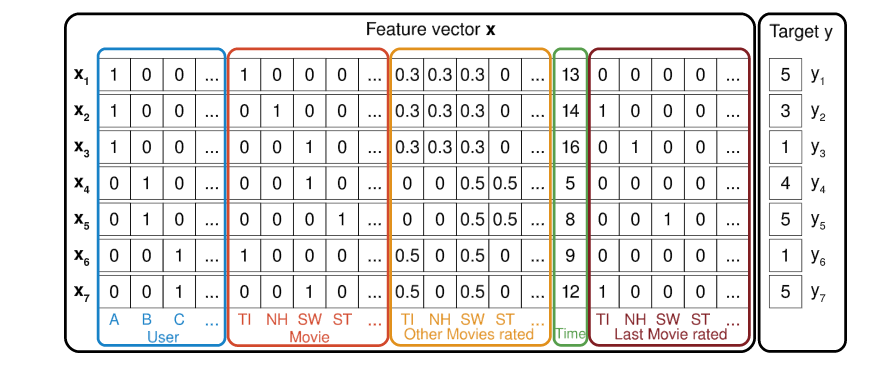
\includegraphics[scale=0.9]{images/featurevectors}
\caption[Feature vector representation in the $SVM^{light}$ format]{Feature vector representation for ratings under the FM models (Source: Factorization machines\cite{rendle2010factorization})}
\label{fig:featurevector}
\end{figure}

\section{Results}

\chapter{General Conclusions}
\label{chapterlabel4}

\addcontentsline{toc}{chapter}{Appendices}

% The \appendix command resets the chapter counter, and changes the chapter numbering scheme to capital letters.
%\chapter{Appendices}
\appendix
\chapter{An Appendix About Stuff}
\label{appendixlabel1}
(stuff)

\chapter{Another Appendix About Things}
\label{appendixlabel2}
(things)

\chapter{Colophon}
\label{appendixlabel3}
\textit{This is a description of the tools you used to make your thesis. It helps people make future documents, reminds you, and looks good.}

\textit{(example)} This document was set in the Times Roman typeface using \LaTeX\ and Bib\TeX , composed with a text editor. 
 % description of document, e.g. type faces, TeX used, TeXmaker, packages and things used for figures. Like a computational details section.
% e.g. http://tex.stackexchange.com/questions/63468/what-is-best-way-to-mention-that-a-document-has-been-typeset-with-tex#63503

% Side note:
%http://tex.stackexchange.com/questions/1319/showcase-of-beautiful-typography-done-in-tex-friends 
% You could separate these out into different files if you have
%  particularly large appendices.

% This line manually adds the Bibliography to the table of contents.
% The fact that \include is the last thing before this ensures that it
% is on a clear page, and adding it like this means that it doesn't
% get a chapter or appendix number.
\addcontentsline{toc}{chapter}{Bibliography}

% Actually generates your bibliography.
\bibliography{bibliography}

% All done. \o/
\end{document}
